\documentclass{article}
\usepackage{graphics}
\usepackage{graphicx}
\usepackage{float}
\usepackage{multicol}

\title{Datascience Homework 6}
\author{Ali Asghar Yousuf - ay06993}
\date{\today}

\begin{document}
\maketitle

\section{Create Database}
\begin{figure}[H]
    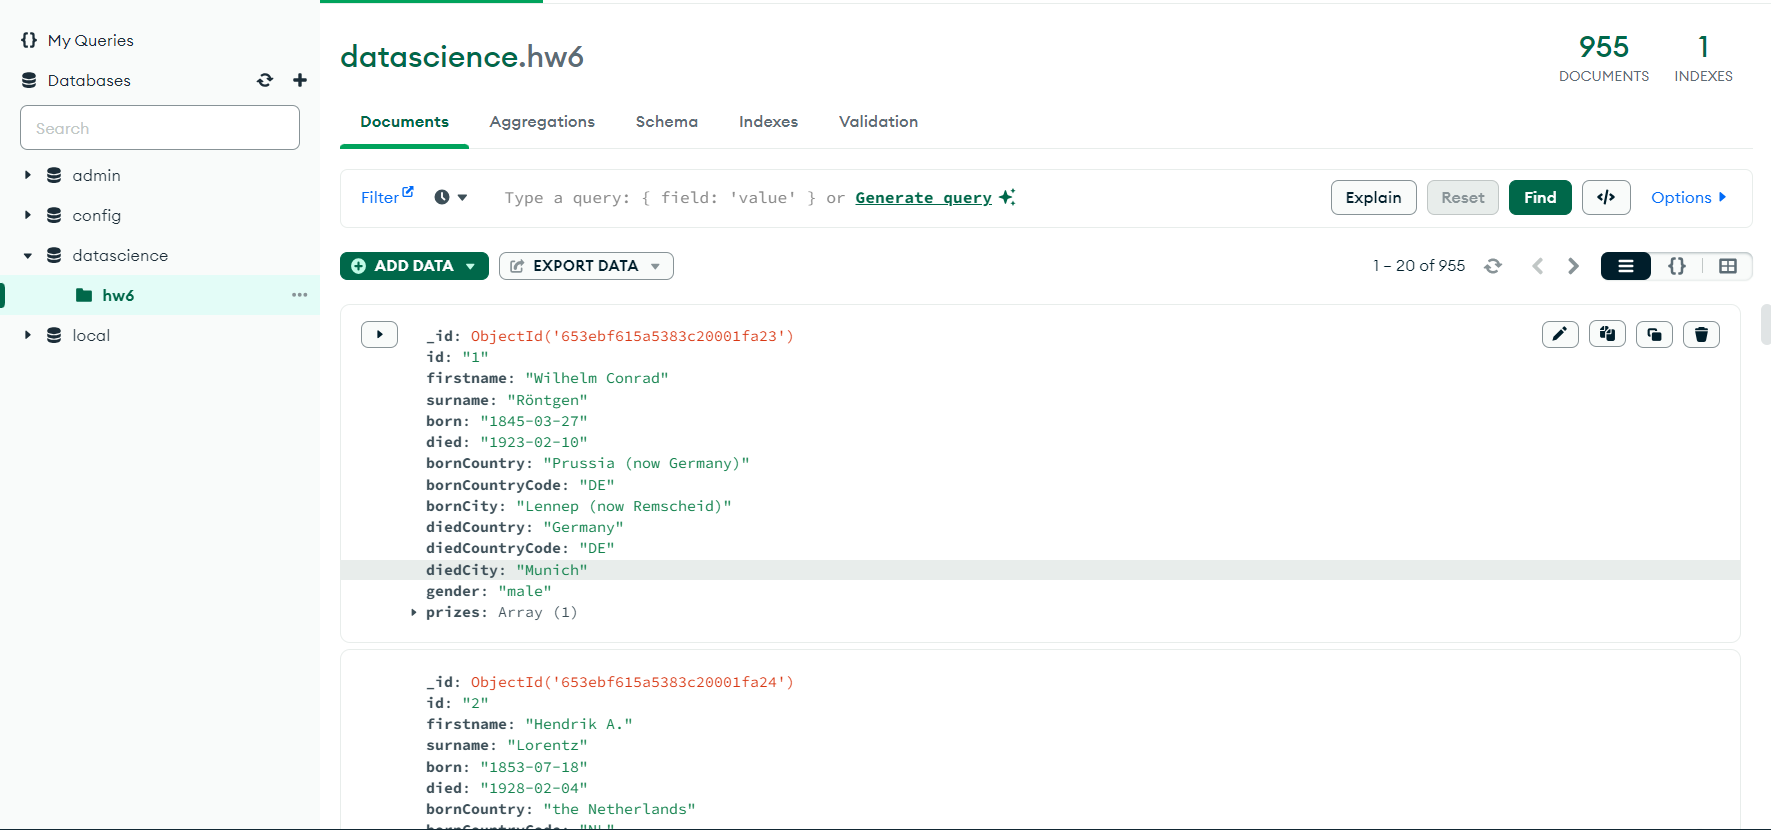
\includegraphics[width=\textwidth]{images/createdb.png}
\end{figure}

\section{Query}
\subsection{Query 1}
The count of total number of records in the collection.

\begin{multicols*}{2}
    \begin{verbatim}
    db.hw6.count()
\end{verbatim}
    \columnbreak

    \begin{figure}[H]
        
\includegraphics[width=0.2\textwidth]{images/q1.png}
    \end{figure}
\end{multicols*}

\subsection{Query 2}
The count of records for each diedCountryCode in descending order of count.

\begin{verbatim}
    db.hw6.aggregate([
        {
            $group: {
                _id: "$diedCountryCode",
                count: { $sum: 1 }
            }
        },
        {
            $sort: { count: -1 }
        }
    ])
\end{verbatim}

\begin{multicols*}{3}
    \begin{figure}[H]
        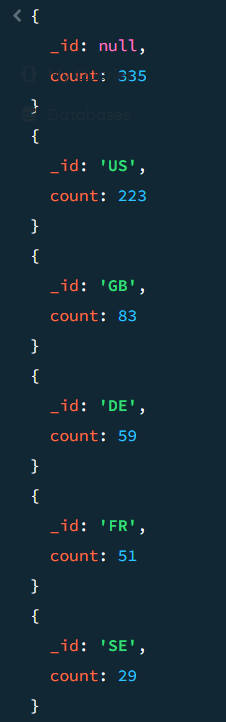
\includegraphics[width=0.3\textwidth]{images/q2a.png}
    \end{figure}

    \columnbreak

    \begin{figure}[H]
        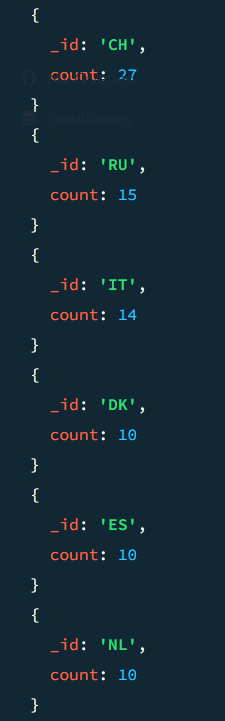
\includegraphics[width=0.3\textwidth]{images/q2b.png}
    \end{figure}

    \columnbreak

    \begin{figure}[H]
        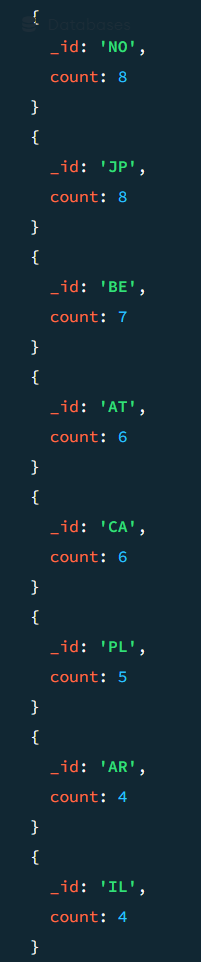
\includegraphics[width=0.2\textwidth]{images/q2c.png}
    \end{figure}
\end{multicols*}

\subsection{Query 3}
The count of records for each prizes.category in descending order of count\dots

\begin{verbatim}
    db.hw6.aggregate([
        {
            $group: {
                _id: "$prizes.category",
                count: { $sum: 1 }
            }
        },
        {
            $sort: { count: -1 }
        }
    ])
\end{verbatim}

\begin{multicols*}{2}
    \begin{figure}[H]
        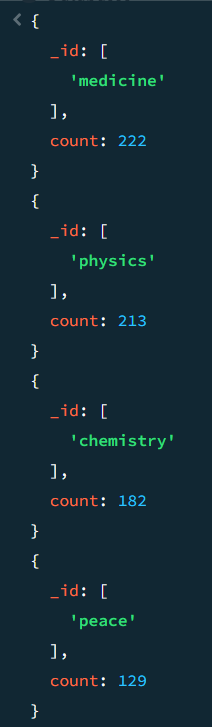
\includegraphics[width=0.3\textwidth]{images/q3a.png}
    \end{figure}

    \columnbreak

    \begin{figure}[H]
        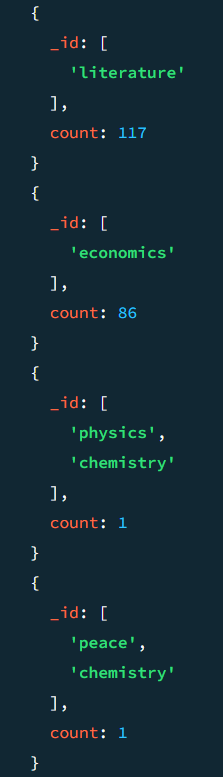
\includegraphics[width=0.3\textwidth]{images/q3b.png}
    \end{figure}
\end{multicols*}

\subsection{Query 4}
The count of records for each gender, diedCountryCode, prize.category when
prize.category is ``Physics''. Order the output by diedCountryCode.

\begin{verbatim}
    db.hw6.aggregate([
        {
            $match: { "prizes.category": "physics" }
        },
        {
            $group: {
            _id: {
                gender: "$gender",
                diedCountryCode: "$diedCountryCode",
                prizeCategory: "$prizes.category"
            },
            count: { $sum: 1 }
            }
        },
        {
            $sort: {
            "_id.diedCountryCode": 1
            }
        }
    ])
\end{verbatim}

\begin{multicols*}{3}
    \begin{figure}[H]
        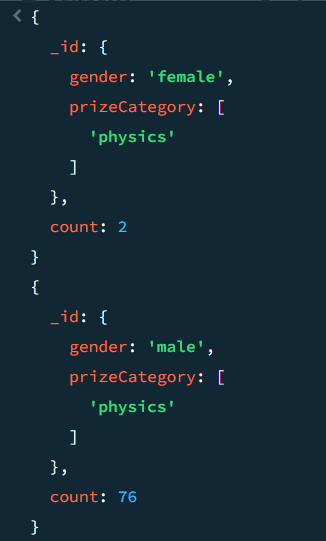
\includegraphics[width=0.3\textwidth]{images/q4a.png}
    \end{figure}

    \columnbreak

    \begin{figure}[H]
        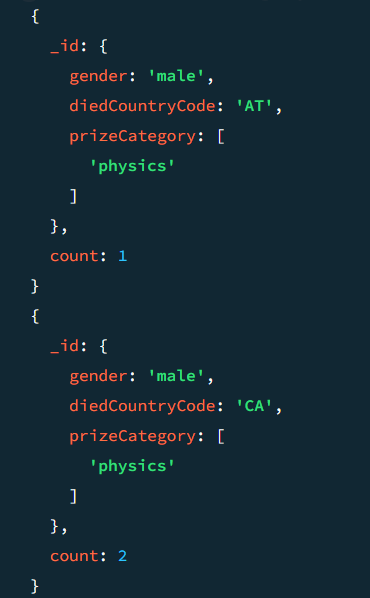
\includegraphics[width=0.3\textwidth]{images/q4b.png}
    \end{figure}

    \columnbreak

    \begin{figure}[H]
        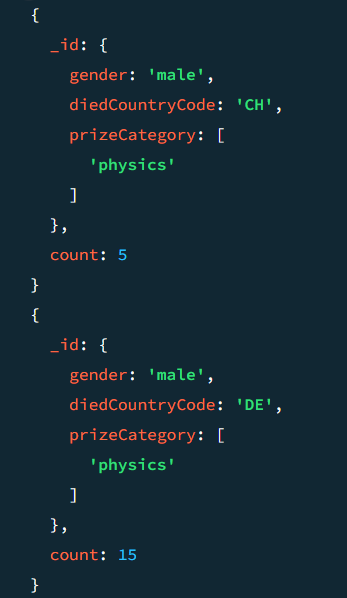
\includegraphics[width=0.3\textwidth]{images/q4c.png}
    \end{figure}
\end{multicols*}

\subsection{Query 5}
Come up with your own query to show any interesting insight. Use atleast two
fields for match and two fields for group.

\begin{verbatim}
    db.hw6.aggregate([
        {
            $match: {
                "diedCountryCode": "FR",
                "bornCountryCode": "FR"
            }
        },
        {
            $group: {
                _id: {
                    gender: "$gender",
                    prizeCategory: "$prizes.category"
                },
                count: { $sum: 1 }
            }
        },
        {
            $sort: { 
                "_id.bornCountryCode": 1,
            }
        }
    ])
\end{verbatim}

\begin{multicols*}{3}
    \begin{figure}[H]
        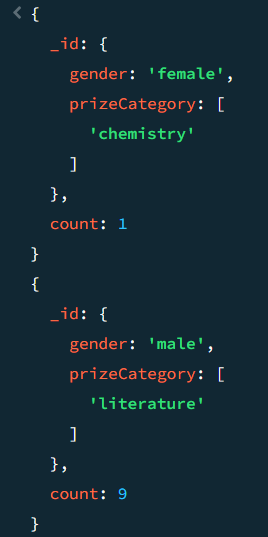
\includegraphics[width=0.3\textwidth]{images/q5a.png}
    \end{figure}

    \columnbreak

    \begin{figure}[H]
        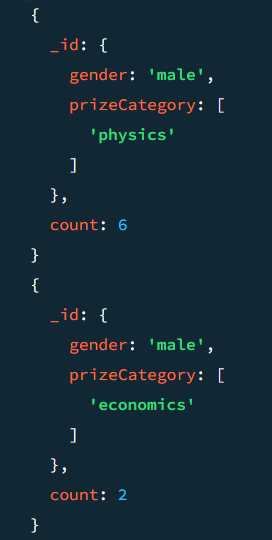
\includegraphics[width=0.3\textwidth]{images/q5b.png}
    \end{figure}

    \columnbreak

    \begin{figure}[H]
        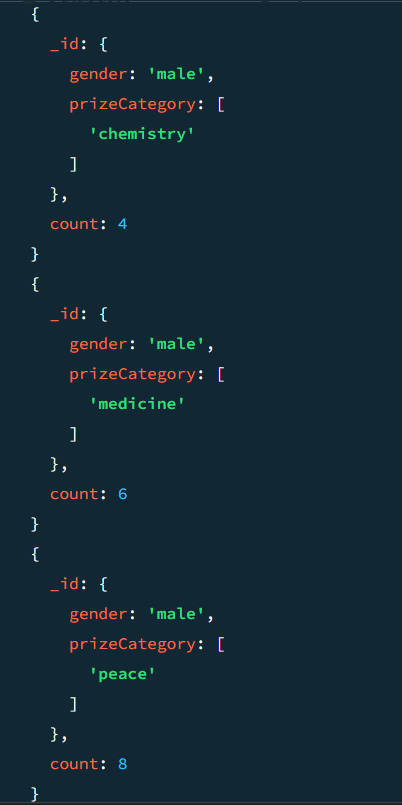
\includegraphics[width=0.3\textwidth]{images/q5c.png}
    \end{figure}
\end{multicols*}

\end{document}